This subsection further explores the possibility that measurement error in education biases the main finding of rising mortality among the least educated whites. High school graduation rates on death certificates are thought to be inflated on average, though higher education levels appear to be reported accurately \citep{Sorlie1996}.  There is no evidence that this bias has changed during the sample period, but (as discussed in Appendix~\ref{sec:app_cps_cohorts}) if overreporting of high school completion on death certificates (but not in the CPS) were to decline over time, it would cause mortality change among high school dropouts to biased upward.

For measurement error to explain the rising mortality among dropouts described in this paper, it would need to be the case: (i) that the measurement error in education changes substantially during the sample period; (ii) that measurement error changes differentially for deaths of deaths of despair and deaths in other categories, at different ages, but changes considerably less for deaths of despair; and (iii) that measurement error has declined dramatically for non-Hispanic whites, but has changed only minimally for blacks. Misreporting rates would have to differ substantially across age groups as well---for example, we find that dropouts account for nearly all mortality gain among 50--54-year-olds white women, but that rising mortality is equally distributed among dropouts and high school graduates among 25--29-year-old white women.  

In contrast, if white respondents were increasingly inflating their education in the CPS, we would expect a uniform increase in mortality from all causes, across all ages, which is not remotely what we find. Note also that other researchers have noted rising health disparities between dropouts and high school graduates, in datasets where misreporting of education is unlikely to be a concern \citep{Montez2011}.

We show here that even if one treats the distinction between dropouts and high school graduates as unreliable, the central finding of rising mortality among the least educated remains clear. To show this, we combine dropouts and high school graduates into a single education group, and we estimate mortality change for three constant education percentile bins: (i) percentiles 0-45 (corresponding approximately to dropouts \textit{and} high school graduates in in the middle of the sample period; (ii) percentiles 45-70; and (iii) percentiles 70-100.  Figure~\ref{fig:causes_3ed} shows estimates of mortality change from 1992--94 to 2016--18 for these three groups. We continue to find a dramatic rise in mortality among whites at the bottom of education distribution, though we have defined the bottom more broadly here.  We find that mortality among the bottom 45\% of the education distribution rises over 50\% for white women below 45, rises 0--50\% for women 40-59, and is flat at older ages. Mortality among white men in the bottom 45\% is rising for age groups below 60.

In short, we find significant increases in mortality disparities by education even when we pool high school graduates and high school dropouts.  However, by ignoring the distinction between dropouts and high school graduates, we miss the important difference in causes of death noted in Figure~\ref{fig:mort_causes}---mortality increases outside of the very bottom of the distribution are driven primarily by deaths of despair, but mortality increases in the bottom 10\% are driven by a multitude of causes. Absent evidence that measurement error in death records has changed substantially during the sample period, rising mortality among the least educated 10\% of the population should be taken seriously.

%%%%%%%%%%%%%%%%%%%%%%%%%%%%%%%%%%%%%%%%%%%%%%%%%
% Figure: Causes of Death -- 3 Education Groups %
%%%%%%%%%%%%%%%%%%%%%%%%%%%%%%%%%%%%%%%%%%%%%%%%%
\begin{figure}[H]
  \caption{Change in non-Hispanic White Mortality: 3 Education Groups}
%  \thispagestyle{empty}
  \label{fig:causes_3ed}
  
  \begin{center}
    \vspace{-.6cm} Panel A: Non-Hispanic White Women
  \end{center}
%  \vspace{-1.4cm}
  \begin{center}
    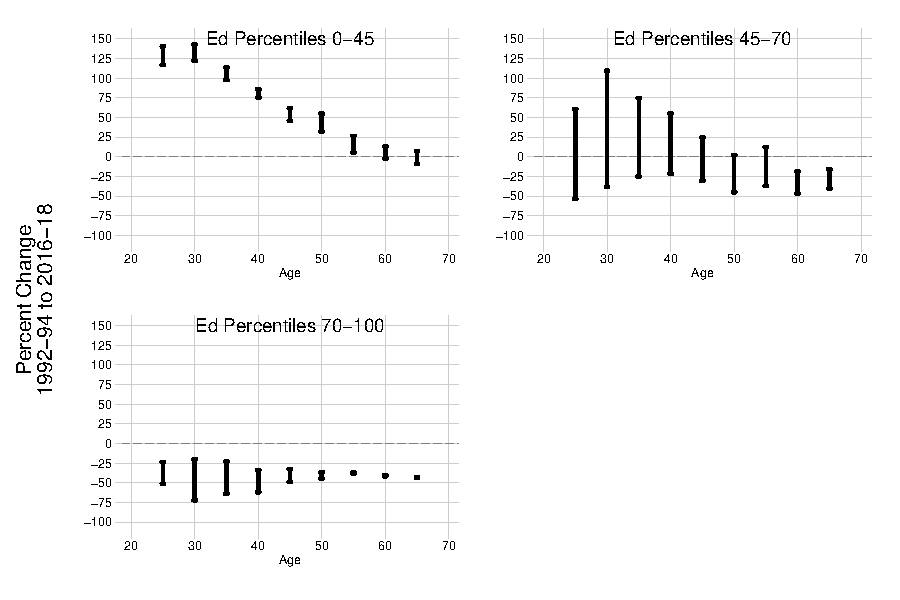
\includegraphics[scale=0.78]{\mortalitypath/causes-ed3-2} &
  \end{center}
  
  \begin{center}
    \vspace{-.6cm} Panel B: Non-Hispanic White Men
  \end{center}
%  \vspace{-1.4cm}
  \begin{center}
    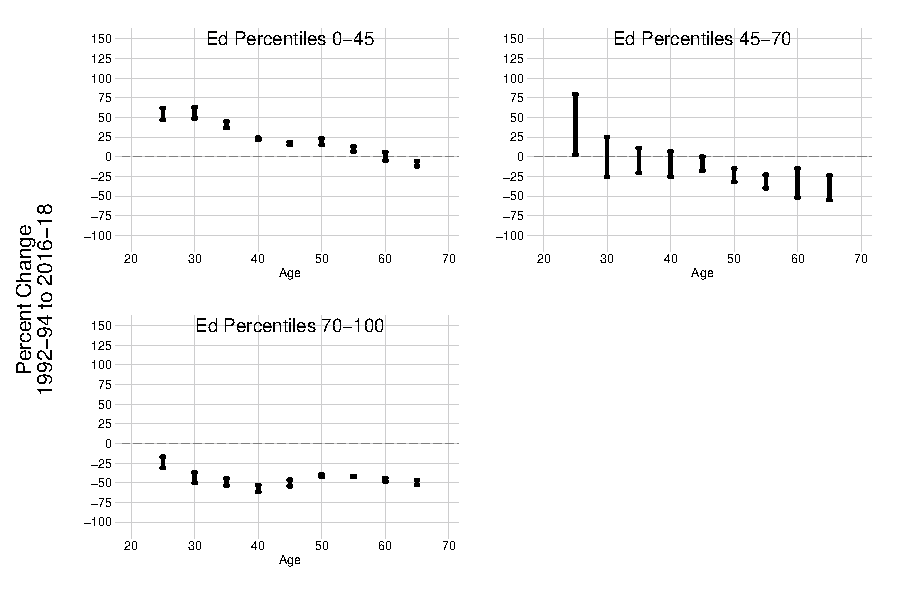
\includegraphics[scale=0.78]{\mortalitypath/causes-ed3-1} \\
  \end{center}
\end{figure}
% \vspace{-1cm}
\tiny{ Note: The graph shows changes in mortality by age, sex, race, and constant percentile education bin. The figure is analogous to Figure \ref{fig:mort_main}, but with the bottom two education categories (percentiles 0--10 and 10--45) pooled into a single category covering percentiles 0--45.  The lines show the bounded set containing the percentage change in the mortality rate from 1992--1994 to 2016--2018 for the given group. Bounds are calculated following Section~\ref{sec:method}. Sources: CPS, NCHS.}
